\documentclass[12pt]{report}
\newcommand{\ThesisTitle}{misure di confidenza per algoritmi di stereo vision}
\newcommand{\ThesisAuthor}{Nicola Dal Lago}
\title{\ThesisTitle}
\author{\ThesisAuthor}
\date{}


%%%%%%%%%%%%%%%%%%%%%%%%%% general %%%%%%%%%%%%%%%%%%%%%%%%%%%%%%%%%%%%%%%%%%
\usepackage{a4}
\usepackage{color,colortbl}         
\usepackage[english,italian]{babel}
\usepackage[T1]{fontenc}
\usepackage[utf8]{inputenc}
\usepackage{indentfirst}          
\usepackage{setspace}
\usepackage{float}

%%%%%%%%%%%%%%%%%%%%%% fonts & symbols  %%%%%%%%%%%%%%%%%%%%%%%%%%%%%%%%%%%%%%
\usepackage{amsmath}
\usepackage{amsmath,mathtools}
\usepackage{amsthm}
\usepackage{amsfonts}
\usepackage{amssymb}
\usepackage{fancyvrb}  
\usepackage{xspace}
\usepackage{times}    
\usepackage[overload]{textcase} 

%%%%%%%%%%%%%%%%%%%%%% Floats %%%%%%%%%%%%%%%%%%%%%%%%%%%%%%%%%%%%%%%%
\usepackage{sidecap}
\usepackage{graphicx}
\usepackage{caption}
\usepackage{subfig}
%\usepackage{subcaption}
\usepackage[algo2e,algochapter,ruled,linesnumbered,vlined]{algorithm2e}

%%%%%%%%%%%%%% page headers and footers %%%%%%%%%%%%%%%%%%%%%%%%%%%%%%
\usepackage{fancyhdr}
\pagestyle{fancy}
\renewcommand{\chaptermark}[1]{
  \markboth{{\bf \chaptername \ \thechapter.} \ #1}{}}
\fancyhead[LE,RO]{\thepage}       
\fancyhead[RE]{\it \small \ThesisTitle }
\fancyhead[LO]{\small \it \leftmark}
\fancyhead[CE,CO]{}                    
\fancyfoot[CE,CO]{}
\fancyfoot[LE,RO]{}
\fancyfoot[RE,LO]{}                    
\renewcommand{\headrulewidth}{1pt}       
\renewcommand{\headheight}{15pt}        
\renewcommand{\footrulewidth}{0pt}      
\addtolength{\headsep}{5mm}

%%%%%%%%%%%%%%%%%%%%% counters %%%%%%%%%%%%%%%%%%%%%%%%%%%%%%%%%%%%%
\setcounter{secnumdepth}{3}
\setcounter{tocdepth}{3}    

%%%%%%%%%%%%%%%% utilities %%%%%%%%%%%%%%%%%%%%%%%%%%%%%%%%%%%%%%%%%%%%
\newcommand{\nullpage}{\newpage\null\thispagestyle{empty}}


\usepackage[
 colorlinks=false,
 a4paper=true,
 linktocpage=true,
 pagebackref=false,
 pageanchor=true,
 hyperindex=true,
 bookmarks=true,
 bookmarksopen=true,
 bookmarksnumbered=true,
 pdffitwindow=true,
 citecolor=blue,
 urlcolor=blue
 ]%
 {hyperref}

\begin{document}

%%----------------------------------- COPERTINA ------------------------------------------------%%

	\setcounter{page}{0}                  %inizia numerazione pagine
	\renewcommand{\thepage}{\roman{page}} %numerazione romana
	\begin{titlepage}
		\begin{center}
			\vbox to0pt{\vbox to\textheight{\vfill 
\includegraphics[width=11.5cm]{./figures/unipd-light} \vfill}\vss}

			\hspace{0.5cm}
			\begin{minipage}{.20\textwidth}
  				
\includegraphics[height=2.5cm]{./figures/unipd-bn}
			\end{minipage}\begin{minipage}{.90\textwidth}
  				\begin{table}[H]
  					\begin{tabular}{l}
  						\scshape{\Large{\bfseries{Università degli Studi di Padova}}} \\
  						\hline \\
  						\scshape{\large{Dipartimento di Ingegneria dell'Informazione}} \\
  					\end{tabular}
  				\end{table}
			\end{minipage}

			\vspace{1.5cm}
			\emph{\Large{Corso~di~Laurea~in~Ingegneria~dell'Informazione}} \\
			
			\vspace{1.5cm}
			\scshape{\Large{\bfseries{\ThesisTitle}}} \\
			\vspace{0.2cm} \linespread{1} \scshape{\large{\bfseries{confidence measures for stereo vision algorithms}}}
		\end{center}

		\vfill
		\begin{normalsize}
			\begin{flushleft}
  
  				\hspace{83pt} \textit{Laureando} \hspace{142pt} \textit{Relatore}\\
  				\vspace{5pt}
  
  				\hspace{62pt} \large{\textbf{Nicola Dal Lago}} \hspace{71pt} \large{\textbf{Prof. Pietro Zanuttigh}}\\
  
  				\vspace{5pt}
  				\hspace{270pt} \textit{Correlatore}\\
  
  				\vspace{5pt}
  				\hspace{247pt} \large{\textbf{Dott. Giulio Marin}}\\
			\end{flushleft}
		\end{normalsize}

		\vfill
		\begin{center}
			\hspace{-0.2cm}
			\line(1, 0){360}

			\textsc{Anno Accademico 2013/2014}
		\end{center}
 	\end{titlepage}


%%------------------------------ ABSTRACT -----------------------------------------%%
	\nullpage                      %pagina bianca

	\chapter*{Abstract}
	\label{sec:Abstract}
	\addcontentsline{toc}{chapter}{Abstract}
	\pagestyle{fancy}
	
	\#TODO: srivere qui l'abstract
	

%%------------------------------ INDICE -------------------------------------------%%
	\nullpage						%pagina bianca			
	\tableofcontents				%indice
	\nullpage						%pagina bianca

	\renewcommand{\thepage}{\arabic{page}} %numerazione normale
	\setcounter{page}{1}                   %inizia numerazione pagine


%%----------------------------- INTRODUZIONE ---------------------------------------%%	
	\chapter{Introduzione}
	\label{sec:Introduzione}
	\pagestyle{fancy}
	
		\section{Stereopsi}
		\label{sec:Stereopsi}
			\textit{
			La stereopsi è la capacità percettiva che consente di unire le immagini provenienti dai due occhi, che a causa del loro diverso posizionamento strutturale, presentano uno spostamento laterale. Questa disparità viene sfruttata dal cervello per trarre informazioni sulla profondità e sulla posizione spaziale dell'oggetto mirato. Di conseguenza la stereopsi permette di generare la visione tridimensionale. \footnote{da \url{https://it.wikipedia.org/wiki/Stereopsi}} \newline}
			
			Si possono quindi identificare due problemi: calcolo delle corrispondenze e triangolazione \cite{fusiello}.\newline
			Il primo consiste nell'accoppiare punti delle due immagini, detti punti coniugati, che sono proiezione dello stesso punto nella scena. Il calcolo delle corrispondenze è un problema possibile in quanto le due immagini differiscono di poco, quindi un punto della scena deve apparire simile nei punti coniugati delle due immagini. Basando solo su questo però, sono possibili molti accoppiamenti sbagliati; le due immagini vengono quindi rettificate prima del calcolo delle corrispondenze, in modo che due punti coniugati si trovino sulla stessa retta (detta retta epipolare). Questo si ottiene ruotando le immagini originali attorno ai loro centri ottici finché i piani 
			focali non diventano co-planari (e quindi anche i piani immagine).\newline
			Per triangolazione si intende il calcolo della distanza tra un punto della scena e il piano formato dalle due fotocamere. Nel caso di due fotocamere parallele ed allineate ci si può facilmente ricondurre alla figura \ref{fig:triangolazione}.
			Fissato come riferimento la fotocamera di sinistra si possono scrivere le equazioni di proiezione prospettica:
			
			\[
			\begin{dcases}
				\frac{f}{z}=\frac{-u}{x} \\
				\frac{f}{z}=\frac{-u'}{x-b}
			\end{dcases}
			\]
			
			\begin{SCfigure}[]
				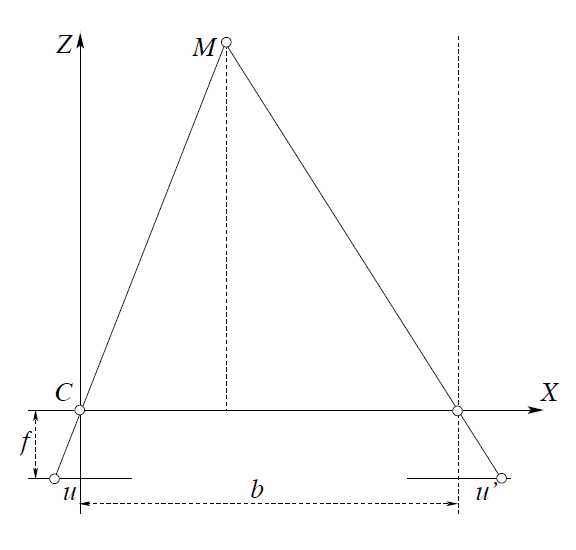
\includegraphics[width=0.6\textwidth]{./figures/Triangolazione_stereoscopica.png}
				\caption{Triangolazione stereoscopica.}
				\label{fig:triangolazione}
			\end{SCfigure}
			
			e risolvendo si ottiene:

			\[
			z=\frac{bf}{u'-u}
			\]
			
			\# TODO frase sbagliata, controlla!!!!!!!!!!!!! \newline
			dove $b$ è la distanza tra i due centri ottici delle fotocamere, $f$ la focale delle fotocamere e $u'-u$ la distanza fra i due centri ottici.
		
		
		\section{Calcolo delle corrispondenze}
		\label{sec:corrispondenze}
		
			Il calcolo delle corrispondenze o della disparità è il problema principale della stereo vision. \newline
			La disparità è la differenza tra due punti coniugati, immaginando di sovrapporre le due immagini. Il calcolo delle corrispondenze non è altro che il calcolo della disparità per ogni pixel delle due immagini \cite{fusiello}. Si ottiene quindi una mappa di disparità del tipo di figura \ref{fig:disparità}.
			
			\begin{figure}
				\centering
				\subfloat[][\emph{Fotocamera di destra}.]
					{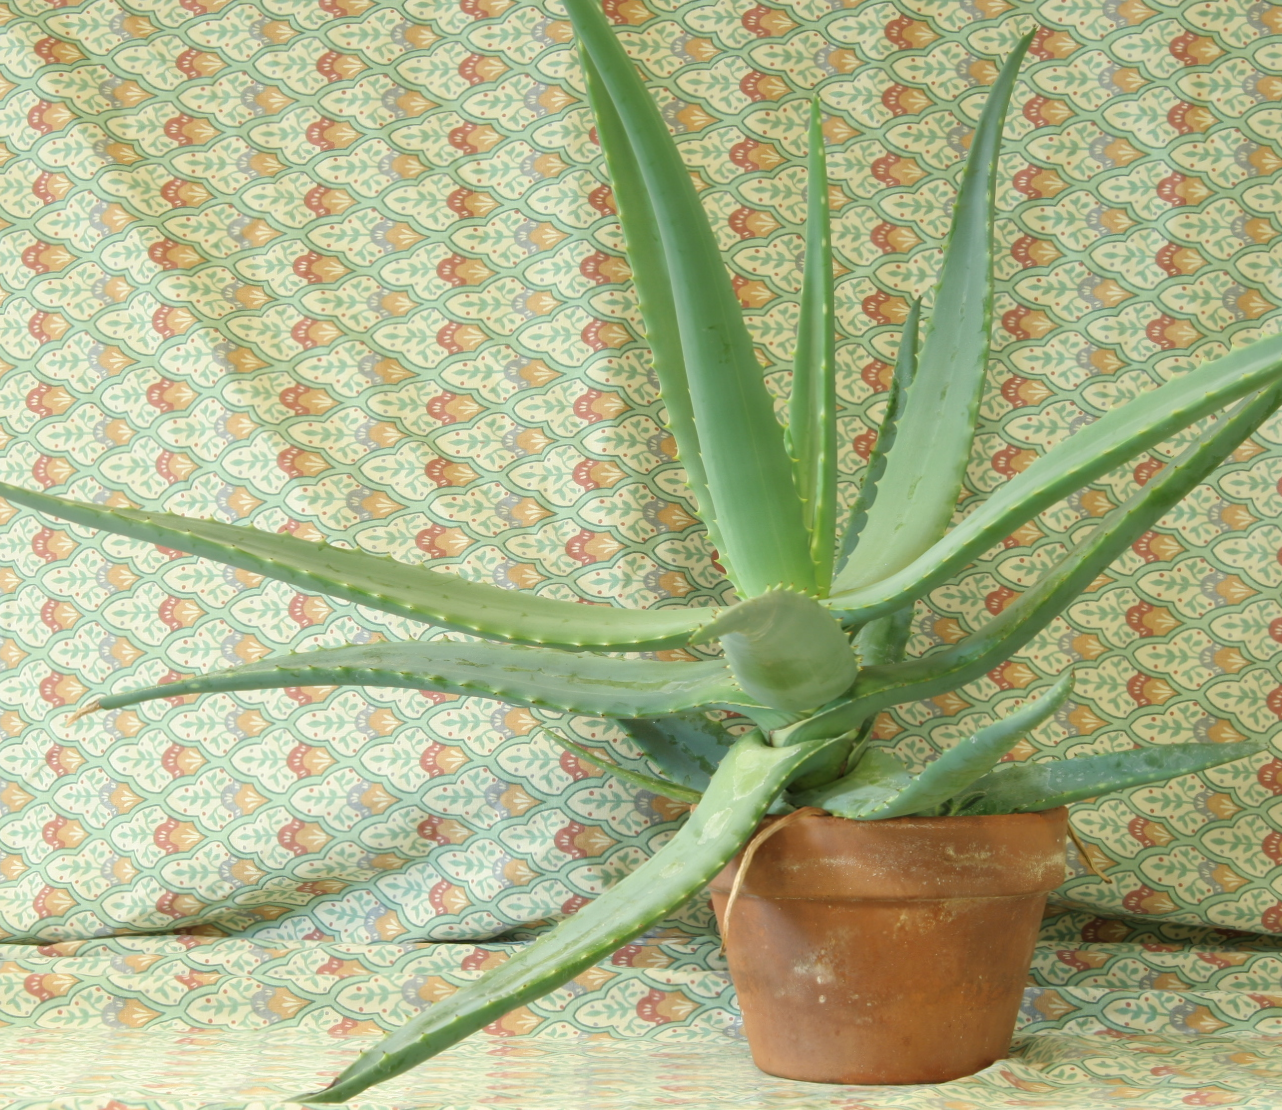
\includegraphics[width=.31\textwidth]{./figures/view1.png}} \quad
				\subfloat[][\emph{Fotocamera di sinistra}.]
					{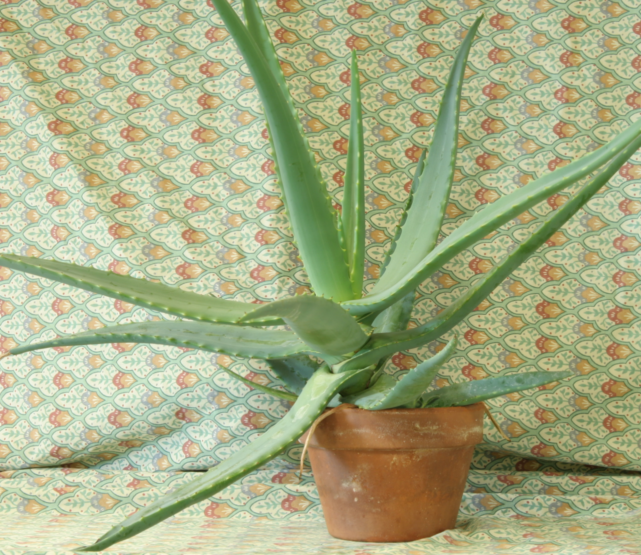
\includegraphics[width=.31\textwidth]{./figures/view5.png}} \quad
				\subfloat[][\emph{Mappa di disparità}.]
					{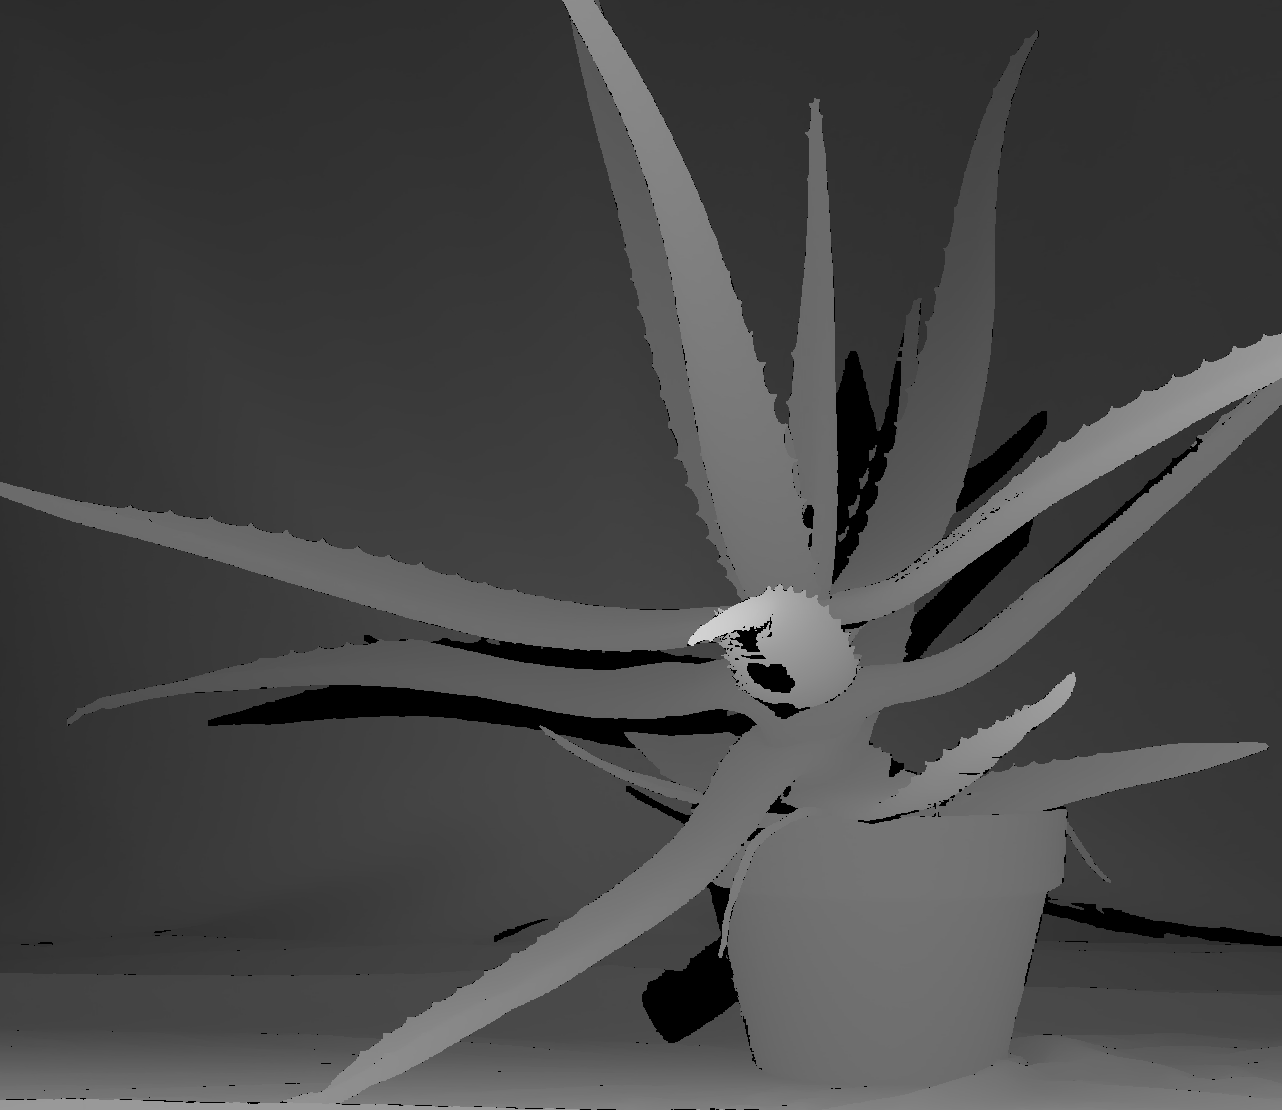
\includegraphics[width=.31\textwidth]{./figures/disp1.png}} 
				\caption{Mappa di disparità con immagine di destra come riferimento, immagine presa da \url{http://vision.middlebury.edu/stereo/data/}}
				\label{fig:disparità}
			\end{figure}
			
						
			
			
			
		
				
%%---------------------------- BIBLIOGRAFIA ----------------------------------------&&
	\begin{thebibliography}{1}
		
		\bibitem{fusiello}
		A. Fusiello,
		\emph{Visione Computazionale, appunti delle lezioni},
		\url{http://profs.sci.univr.it/~fusiello},
		2008.

		\bibitem{mercedes}
		D. Pfeiffer, S. Gehrig, N. Schneider,
		\emph{Exploiting the Power of Stereo Confidences},
		IEEE Conference on Computer Vision and Pattern Recognition, 2013.
	
		\bibitem{mordohai_pami}
		X. Hu, P. Mordohai,
		\emph{A Quantitative Evaluation of Confidence Measures for Stereo Vision},
		IEEE Transactions on Pattern Analysis and Machine Intelligence, 2012.
		
		\bibitem{dataset_2006_1}
		D. Scharstein, C. Pal,
		\emph{Learning conditional random fields for stereo},
		IEEE Computer Society Conference on Computer Vision and Pattern Recognition (CVPR 2007), Minneapolis, MN, June 2007.
		
		\bibitem{dataset_2006_1}
		H. Hirschmüller, D. Scharstein,
		\emph{Evaluation of cost functions for stereo matching},
		IEEE Computer Society Conference on Computer Vision and Pattern Recognition (CVPR 2007), Minneapolis, MN, June 2007.
		
		\bibitem{opencv}
		\emph{OpenCV library 2.4.9},
		\url{http://opencv.org/}.
		
		
	\end{thebibliography}	
	





\end{document}